% chap6.tex (Significance and Future Work)

\chapter{Experiments}

In this section, we evaluate Prov-CPS using our anomaly detection algorithm on a climate control system and an automotive network bus.

\section{Climate Control System}
The experiment evaluation serves as a preliminary study to confirm the correctness of our theoretical approach in detecting anomalous instances between provenance graphs. We evaluate our intrusion detection algorithm on Prov-CPS by implementing an application which simulates a climate control system. Climate control systems ensure a proper functional environment for people and machinery. Constant irregularities in temperature could have devastating effects on industrial machinery. This system consists primarily of a heating ventilation and air conditioning (HVAC) system which uses temperature and humidity data to regulate environmental conditions within a building. We utilize a publicly available dataset \cite{LANGEVIN201594} which consists of a year's worth of longitudinal data on the thermal conditions, related behaviors, and comfort of twenty-four occupants in a medium-sized building generated at  a period of fifteen minutes. We utilize the temperature and humidity data as input to our simulation. We generate provenance graphs for each week of the year. We compare the provenance graph generated in consecutive weeks to see how they differ using our graph similarity approach (i.e., week 1 compared to week 2, week 2 compared to week 3 etc.). 
\par Figure \ref{figure_climate} depicts the cosine similarity between provenance graphs generated from the first occupant by preceding weeks. 

%Ensuring a proper threshold score is used for detection is an important task that requires extensive knowledge of the application domain. The threshold is manually set to a value which is defined by domain experts. For automatic anomaly threshold detection, one can use prediction methods to define an anomaly score. As an example, a threshold might be set to $0.15$ in which all of the scores below the threshold are considered anomalous. 

Since the dataset does not contain attacks, the declines shown in Figure \ref{figure} would likely cause false positives.
 
% This might also be as a result of rapid variation in temperature change for each week in the given dataset.

%The rapid decline in the graph is as a result of anomalies between the provenance graphs. This might be as a result of rapid variation in temperature change for each week in the given dataset.  



\begin{figure}[tb]
\begin{center}
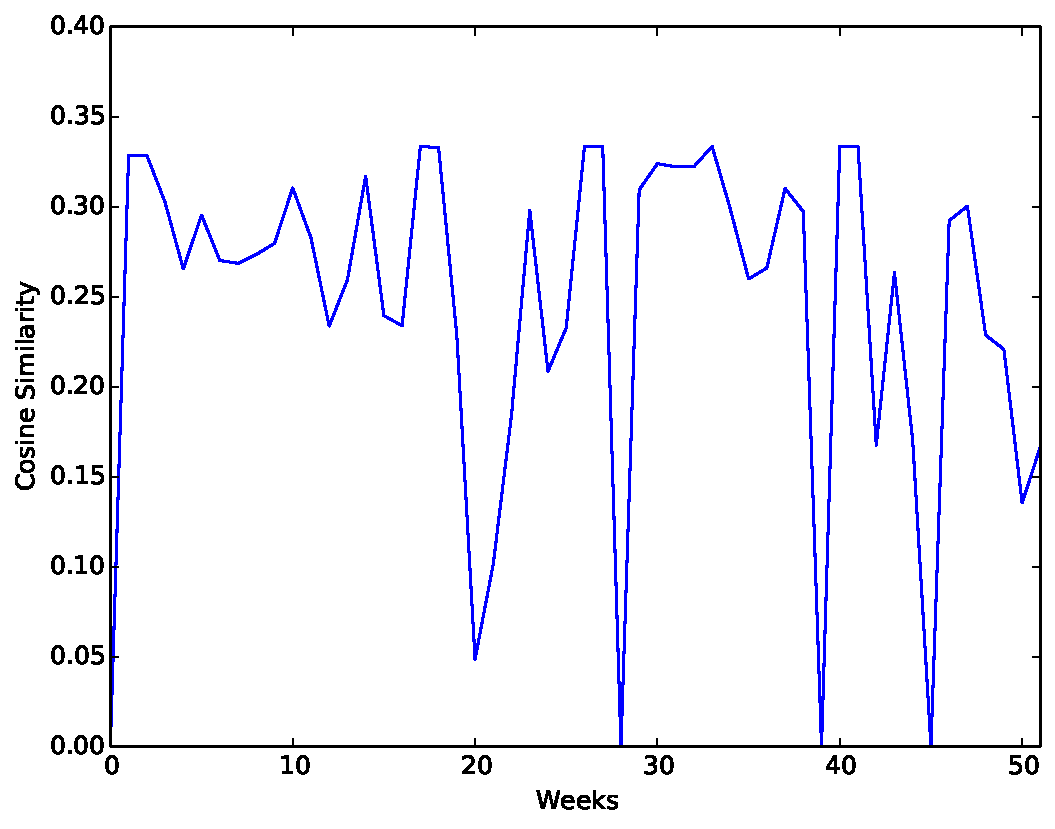
\includegraphics[width=.7\columnwidth]{foo.pdf}
\end{center}
\caption{Provenance graph comparison of climate control system by week.}
\label{figure_climate}
\end{figure}

\section{J1939 Network Bus }

We evaluate Prov-CPS using J1939 CAN data recorded from a Peterbilt truck~\cite{peterbilt}.  This dataset consists of J1939 messages representing normal driving conditions observed on the high speed CAN bus that were logged for a duration of 74 seconds consisting of a total of 16,223 messages.
%
%
%Our experiments calculates the percentage storage savings (i.e., size difference) between the original trace  and the resulting trace file after pruning.
%
%
%\subsection{Target Application: J1939 Network Bus}
The J1939 messaging protocol is an extension of the CAN messaging protocol which is mostly used in heavy-duty trucking vehicles and commercial buses to communicate between in-vehicle electronic control unit (ECUs).  %ECUs are embedded microcontollers contained in vehicles for controlling electrical components. Examples of ECUs are vehicle entertainment systems, engine control module, door control module etc. Each ECU contained in a vehicle listens to messages received on the CAN bus to determine an appropriate message based on the ID parameters. 
A J1939 message consists of a message ID, number of data bytes sent, data, and error checking code. 
%
A J1939 message ID consists of a 29-bit value used to differentiate messages sent by different ECUs. %A message identifier is divided into six categories:  Priority (P), Extended Data Page (EDP), Data Page (DP), PDU format (PF), PDU Specific (PS) and Source Address (SA). SA denotes the origin of the message. 
%An essential component of the message id is the Parameter Group Number (PGN). A PGN is a unique 18 bit identifier used for identifying specific message types. For example the TSC1 messages that determine the engine speed has a PGN value $0000_{16}$. To calculate a PGN number, if the PF value is less than 240, the PGN value can be derived from the combination of the EDP, DP, and PF fields. If the PF field is greater than 240, the PGN field is derived by the combination the P, EDP, DP, PF, and PS components. PGN are further broken down into Suspect Parameter Numbers (SPN) which defines unique data.
For our purposes, we only rely on two fields contained in the message ID: the source address field, which denotes the origin of the message, and the priority field to support priority-based pruning.

From the J1939 dataset, we recreate a trace where each message causes one trace event. We map the source address to the producer identifier in the Prov-CPS model, and map the CAN bus as the controller. The action is a ``receive'' (Rx) activity denoting a passive listener on the bus. We also have the ability to recreate the timestamps from the dataset to be the same in the trace events, but in these experiments we do not use the trace event timestamp. The data object of each trace event consists of the (up to 8) data bytes of the J1939 message. The entire 29-bit message ID is stored as a priority field in the trace event to use for priority-based pruning.

%\subsubsection{\textbf{Malicious Message Injection}} 

Based on the enormous physical constraint that exists in performing real-time message injection attacks on heavy vehicles, and the support of prior work that uses simulation of message injection attacks in CAN networks~\cite{7504089, Otsuka}, we chose to simulate message injection attacks on a CAN bus network. This attack is achieved by recreating the expected log file containing CAN messages received on a CAN bus in an event of a malicious attack. Our message injection attack was modeled after the attacked performed by Mukherjee et al.~\cite{Mukherjee2017APG}. 
%
We simulate message injection attacks by injecting malicious messages into the J1939 dataset using a TSC1 message code, which has a message ID beginning with 21 bits all 0. These messages are used to control the engine's RPM or torque. We inject 10 consecutive TSC1 messages at varied points in the dataset within an existing time gap between two consecutive messages that is greater than 12 times the minimum time gap between two consecutive messages. This is to ensure that we accurately simulate malicious message injection without either time overlap or in excess of the bus bit rate. We chose 10 different log files with the injected attacks in distinctly different regions of the log file (at least 400 messages apart).

For anomaly detection as described in Section~\ref{sec:prov_anomaly}, we take the first quarter of the driving log as a training (observation) set. We do not inject any new messages in this portion of the log, and therefore it is the same in all experiments. The remaining three quarters of the driving log are the test (detection) set, and each anomalous log file contains injected attack messages somewhere in that set. We further divide the training and test sets into equal-sized windows, where the window size is a fraction $f$ of the number of messages in the training set, that is, each window has size equal to $f * n/4$ where $n$ is the number of messages in the log file, i.e., 16,223. A provenance graph is generated for each window, and so the window size is varied as a parameter to explore the effect that scaling graph size has on the performance of the anomaly detector. Performance is measured by collecting the number of true negatives (TN), true positives (TP), false negatives (FN), and false positives (FP) and calculating the true positive rate (TPR) and false positive rate (FPR) in the usual way as:
\[TPR = \frac{TP}{TP+FN}\quad FPR = \frac{FP}{FP+TN}\]
For each window size, i.e., for each different value of $f$, we provide a cumulative TPR and FPR based on the sum of all the positives and negatives recorded over multiple variations of the log file. 


\begin{table*}[tb!] \centering

\caption{Cumulative results of anomaly detection true negative (TN), true positive (TP), false negative (FN), and false positive (FP) for no pruning, FIFO-based pruning, and prioritized pruning based on application priority values.}\label{tab:results}

\begin{tabular}{c|cccc|cccc|cccc}
\textbf{Window Size} & \multicolumn{4}{|c}{\bf No Pruning} & \multicolumn{4}{|c}{\bf FIFO Pruning} & \multicolumn{4}{|c}{\bf Priority Pruning} \\
\textbf{(Messages)} & \textbf{TN} & \textbf{TP} & \textbf{FN} & \textbf{FP} & \textbf{TN} & \textbf{TP} & \textbf{FN} & \textbf{FP} & \textbf{TN} & \textbf{TP} & \textbf{FN} & \textbf{FP}\\ \midrule
15 & 7310 & 13 & 4 & 353 & 7638 & 9 & 8 & 25  & 7607 & 13 & 4 & 56 \\ 
20 & 5609 & 11 & 4 & 376 & 5829 & 8 & 7 & 156  & 5764 & 14 & 1 & 221  \\ 
30 & 3605 & 10 & 3 & 382 & 3788 & 7 & 6 & 199 & 3808 & 9 & 4 & 179 \\ 
40 & 2461 & 12 & 2 & 525  & 2795 & 4 & 10 & 191  & 2658 & 12 & 2 & 328\\ 
50 & 1713 & 9 & 2 & 676 & 2179 & 7 & 4 & 210 & 1971 & 11 & 0 & 418\\ 
126 & 492 & 10 & 0 & 458 & 619 & 5 & 5 & 331 & 591 & 10 & 0 & 359 \\ 
253 & 138 & 11 & 0 & 331 & 201 & 8 & 3 & 268 & 108 & 11 & 0 & 361 \\ 
506 & 9 & 11 & 0 & 220  & 25 & 10 & 1 & 204 & 0 & 11 & 0 & 229 \\ 
1013 & 9 & 11 & 0 & 100 & 0 & 11 & 0 & 109 & 0 & 11 & 0 & 109 \\
\end{tabular}

\end{table*}

%\begin{table*}[] \centering
%%\ra{1.3}
%
%\begin{tabular}{@{}llllr@{}}\toprule
%\textbf{F} & \textbf{True Negative} & \textbf{True Positive} & \textbf{False Negative} & \textbf{False Positive}\\ \midrule
%\textbf{0.00391} & 7638 & 9 & 8 & 25 \\ \hdashline
%\textbf{0.00500} & 5829 & 8 & 7 & 156 \\ \hline
%\textbf{0.00750} & 3788 & 7 & 6 & 199 \\ \hline
%\textbf{0.0100} & 2795 & 4 & 10 & 191 \\  \hline
%\textbf{0.0125} & 2179 & 7 & 4 & 210 \\ \hline
%\textbf{0.0313} & 619 & 5 & 5 & 331 \\ \hline
%\textbf{0.0625} & 201 & 8 & 3 & 268 \\ \hline
%\textbf{0.125} & 25 & 10 & 1 & 204 \\ \hline
%\textbf{0.250} & 0 & 11 & 0 & 109 \\  \midrule
%
%\bottomrule
%\end{tabular}
%
%\caption{Experimental Results of TP, TN, FP, and FN rates without pruning with FIFO pruning}
%\end{table*}
%
%\begin{table*}[] \centering
%%\ra{1.3}
%
%\begin{tabular}{@{}llllr@{}}\toprule
%\textbf{F} & \textbf{True Negative} & \textbf{True Positive} & \textbf{False Negative} & \textbf{False Positive}\\ \midrule
%\textbf{0.00391} & 7634 & 3 & 14 & 29 \\ \hdashline
%\textbf{0.00500} & 5853 & 4 & 11 & 132 \\ \hdashline
%\textbf{0.00750} & 3974 & 2 & 11 & 13 \\ \hdashline
%\textbf{0.0100} & 2919 & 3 & 11 & 67 \\  \hdashline
%\textbf{0.0125} & 2319 & 4 & 7 & 70 \\ \hdashline
%\textbf{0.0313} & 735 & 2 & 8 & 215 \\ \hdashline
%\textbf{0.0625} & 337 & 2 & 9 & 132 \\ \hdashline
%\textbf{0.125} & 160 & 1 & 10 & 69 \\ \hdashline
%\textbf{0.250} & 54 & 1 & 10 & 55 \\  \midrule
%
%\bottomrule
%\end{tabular}
%
%\caption{Experimental Results of TP, TN, FP, and FN rates without pruning with Priority pruning}

%\end{table*}

%\begin{figure*}[!htb]
%   \begin{minipage}{0.48\textwidth}
%     \centering
%     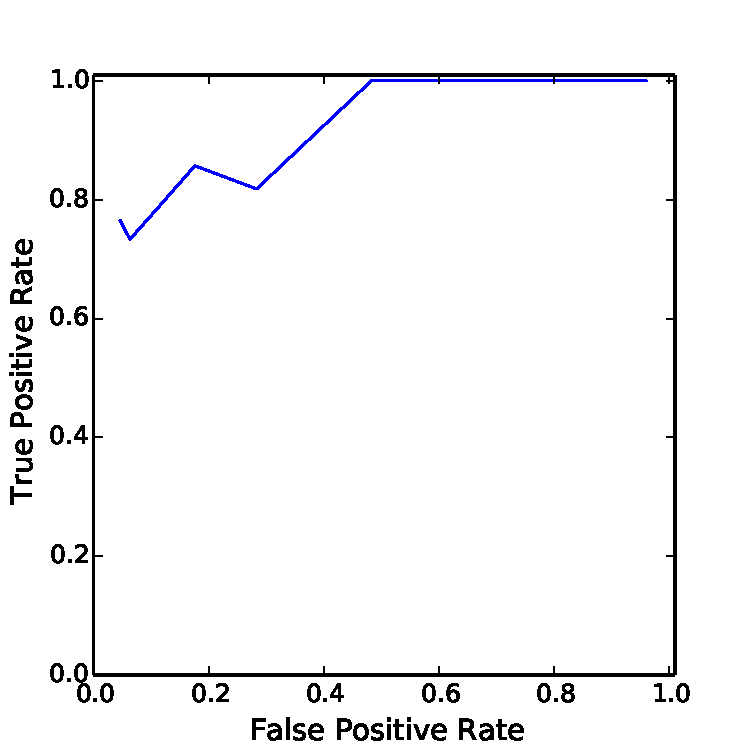
\includegraphics[width=.7\linewidth]{roc_curve_0.pdf}
%     \caption{Interpolation for Data 1}\label{Fig:ROC without Pruning}
%   \end{minipage}\hfill
%   \begin {minipage}{0.48\textwidth}
%     \centering
%     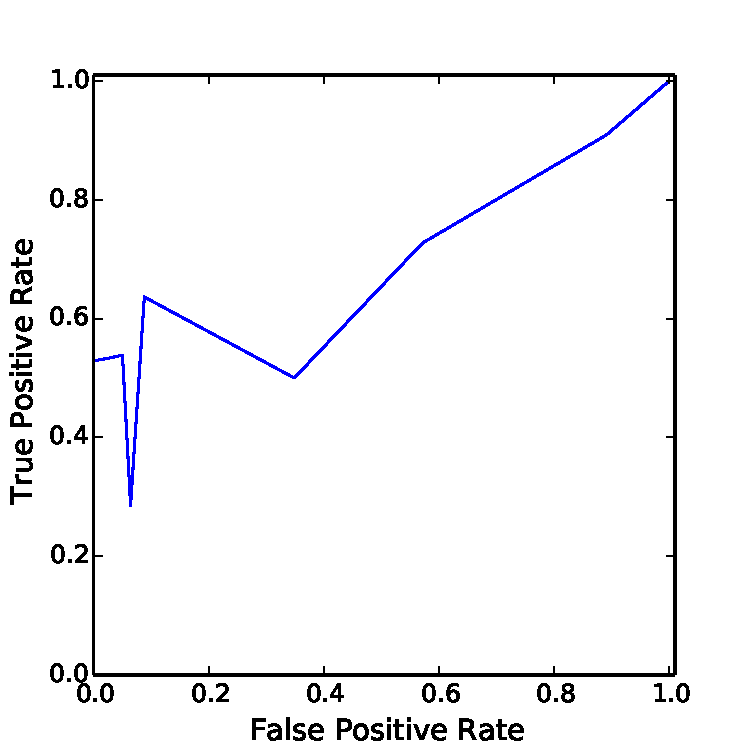
\includegraphics[width=.7\linewidth]{roc_curve_1.pdf}
%     \caption{Interpolation for Data 2}\label{ROC with Pruning}
%   \end{minipage}
%\end{figure*}


\begin{figure*}[!htb]
 
\centering
\subfloat[ROC with No Pruning]{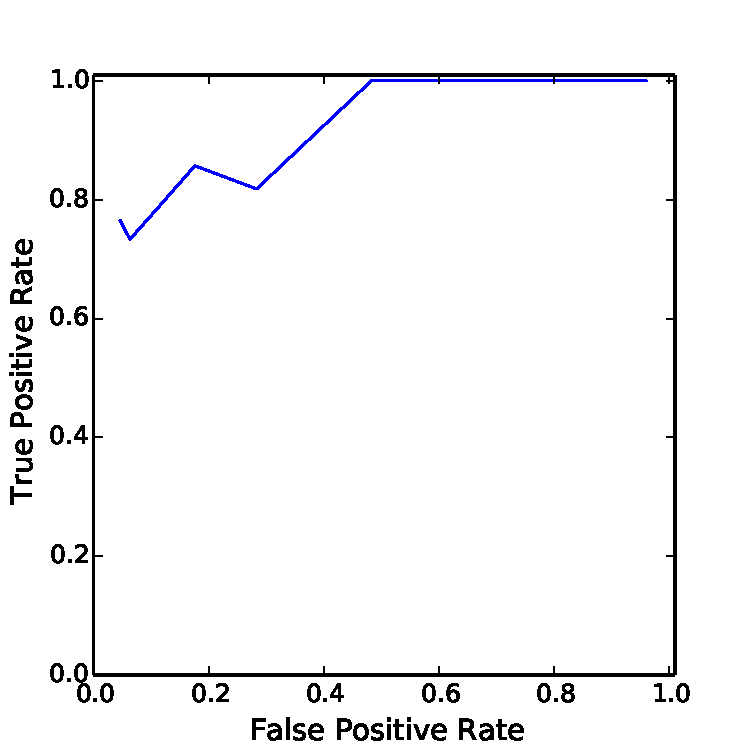
\includegraphics[width=.3\textwidth]{roc_curve_0.pdf}\label{fig:roc_curve_0}}
\hfill
\subfloat[ROC with FIFO Pruning]{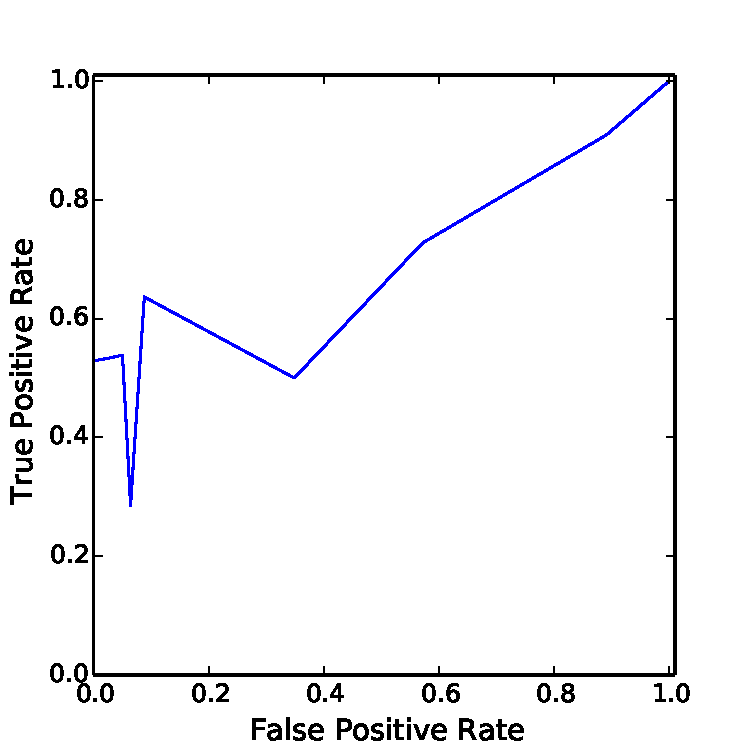
\includegraphics[width=.3\textwidth]{roc_curve_1.pdf}\label{fig:roc_curve_1}}
\hfill
\subfloat[ROC with Priority Pruning]{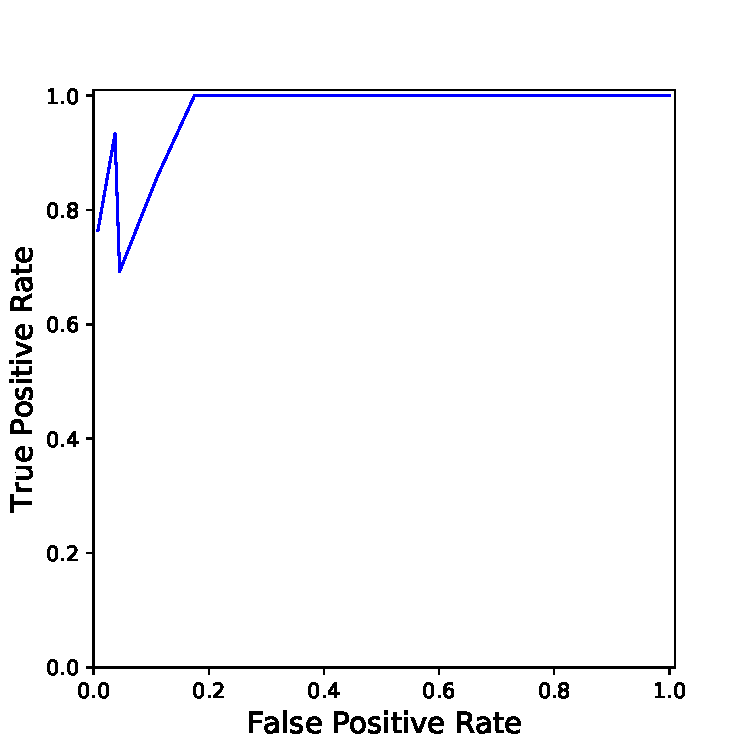
\includegraphics[width=.3\textwidth]{roc_curve_2.pdf}\label{fig:roc_curve_2}}
\caption{Receiver operating characteristic (ROC) curves without pruning and with FIFO or Priority pruning.}
\label{fig:roc}

\end{figure*}


Table~\ref{tab:results} shows the cumulative results of anomaly detection summed over 10 log files each containing 1 set of 10 injected messages. Each approach to pruning---no pruning, FIFO pruning, and priority pruning---was evaluated using the same input log files.  For the pruning algorithms, we chose to prune one-half of the window size for these experiments. Each row shows a different window size, which corresponds to a different value of $f$ ranging between 0.0039 to 0.25 with corresponding window sizes between 15 and 1013 messages. Cumulative results also are presented using a receiver operating characteristic (ROC) curve showing how performance changes with $f$. Figure~\ref{fig:roc} shows the ROC curve for each pruning algorithm (no pruning, FIFO pruning, and priority-based pruning) separately evaluated in the same way using the same modified datasets. As $f$ increases, the window sizes get larger and so do the graphs, which increases their relative variability and therefore decreases the similarity scores, thus resulting in higher TPR and FPR. With smaller $f$ and therefore small graphs, the anomaly detection algorithm is better able to match the features of graphs in the training and testing sets, so TPR can stay high while FPR decreases; note that with smaller window sizes, there are also more decisions (positives and negatives) to make. 

